\usetikzlibrary{shapes.geometric}
\usetikzlibrary{positioning}

\newcommand{\apparatus}[4]{\node[square node] (#1) at (#2,#3){#4};
                           \node[port] (#1+) at (#2 + 0.375, #3 + 0.5){+};
                           \node[port] (#1-) at (#2 + 0.375, #3 - 0.5){-};}

\chapter{Postulates of Quantum Mechanics}

We first consider the mathematical objects used to model physical systems and variables. By comparing the objects used in classical and quantum mechanics, we make sense of the first three postulates of quantum mechanics. Then, we compare the Copenhagen and von Neumann descriptions of measurement and their relation to the fourth and fifth postulates.

\section{Physical Variables and State Spaces}
\subsection{Classical States}
Consider the spin of an electron. Treating the electron as a classical system, its spin state is modeled by a vector $\vec{S} \in \mathbb{R}^3$:
\begin{align}
\vec{S} = (S_x, S_y, S_z)
\end{align}

Each component $S_{x_i}$ is a physical variable representing the magnitude of spin oriented in the $\hat{x_i}$ direction.

$\vec{S}$ has the capacity to determine spin in any direction using the inner product of the state space $\mathbb{R}^3$:
\begin{align}
S_n(S) = \vec{S} \cdot \hat{n}
\end{align}

We see that in classical mechanics, physical variables are modeled using functions. Each function $S_n$ maps a spin state $[\vec{S}$ to a real scalar representing the spin of the electron aligned along the $\hat{n}$ axis.

What makes classial mechanics familiar to everyday experience boils down to intuitive but important properties of the state space $\mathbb{R}^3$:
\begin{itemize}
\item For any direction $\hat{n}$, $\vec{S}$ determines spin $S_n$
\item $S_n$ can be any real value
\end{itemize}

$\vec{S}$ determines spin in any direction because TODO. Consequently, the sample spaces for spin in any two directions $\hat{n}$ and $\hat{m}$ are \textit{compatible}, meaning that $S_n$ and $S_m$ may be simultaneously determined. Spin states in $\mathbb{R}^3$ are interpreted physically as the electron posessing definite values for every $S_n$ at some instant in time.

In addition to spin states determing all $S_n$, the state space allows $S_n$ to take on any real value. There are no fundamental restrictions on which real numbers $S_n$ could be; its sample space is continuous and infinitely large.

\subsection{Quantum States}
Measurements of electron spin show that the intuitive classical properties do not hold. Recall that only two magnitudes of spin have ever been measured. $S_n$ is a \textit{quantized} physical variable; its sample space is discrete and finite.

Second, the results of successive measurements of a spin system imply that $\vec{S}$ does not determine spin in some general direction $S_n$. Recall the results of succesively measuring spin in orthogonal directions discussed in TODO REF. After measuring $S_x$, $\vec{S}$ appears to ``forget'' a previous measurement of $S_z$. All we may know about the system at one instant in time is spin in one direction. The inabilitiy to simultaneously determine spin in two independent directions $\hat{n}$, $\hat{m}$ should be reflected through $S_n$ and $S_m$ having \textit{incompatible} sample spaces.

Electron spin measurements violate the intuitive classical state space properties mentioned in 3.1.1. In response, we must change the mathematical objects used to represent system states and physical variables. Specifically, the sample space of $S_n$ must restrict observable values to spin up and spin down, and $S_n$ and $S_m$ should have incompatible sample spaces. In combination, the first three postulates of quantum mechanics take care of these differences.

Quantum mechanics postulates that a system's state is completely described by a normalized vector in a linear state space.

\invisiblesubsubsection{Postulate 1 (Hilbert Space)}
\begin{Thm:Postulate}{1}
    The state of a physical system is defined by specifying an abstract vector $\ket{\psi}$ in a Hilbert state space $\mathcal{H}$.
\end{Thm:Postulate}

For spin-$\frac{1}{2}$ systems such as electrons, the two-dimensional Hilbert space consists of all linear combinations of spin-up and spin-down:
\begin{equation}
  \ket{\psi} \in \mathcal{H} \\ \nonumber
  \ket{\psi}\{\alpha\ket{+_{S_z}} + \beta\ket{-_{S_z}}\}
\end{equation}
where $\alpha, \beta \in \mathbb{C}$.

$\mathcal{H}$ is an abstract state space; components of $\ket{\psi}$ cannot be interpreted as physical variables as they are for the classical spin state $S$. So, we introduce physical meaning with more postulates.

\invisiblesubsubsection{Postulate 2 (Physical Variables as Operators)}
The second posulate of quantum mechanics states that physical variables are described by linear operators:
\begin{Thm:Postulate}{2}
    Every physical variable $\mathcal{A}$ is described by an operator $A$ acting in $\mathcal{H}$.
\end{Thm:Postulate}

\invisiblesubsubsection{Postulate 3 (Observable Values)}
Justifying the second postulate is easiest when also considering the third postulate:
\begin{Thm:Postulate}{3}
    The only possible result of the measurement of a physical variable $\mathcal{A}$ is one of the eigenvalues of the corresponding operator $A$.
\end{Thm:Postulate}

The operator correlates elements of a finite sample space (eigenvalues) with particular system states (eigenstates). Consequently, a state can only be interpreted as having a definite variable value if it is an eigenstate of that variable's operator. To illustrate this, consider the operator representing $S_z$. Written in the basis of its own eigenstates,
\begin{align}
    S_z \doteq \frac{\hbar}{2}\begin{bmatrix} 1 & 0 \\ 0 & -1 \end{bmatrix}
\end{align}
This operator correlates $z$ spin-up $\left(S_z = \frac{\hbar}{2}\right)$ with eigenstate
\begin{align}
    \ket{\psi} = \ket{+_{S_z}} \doteq \begin{bmatrix} 1 \\ 0 \end{bmatrix}
\end{align}
and $z$ spin-down $\left(S_z = \frac{-\hbar}{2}\right)$ with eigenstate
\begin{align}
    \ket{\psi} = \ket{-_{S_z}} \doteq \begin{bmatrix} 0 \\ 1 \end{bmatrix}
\end{align}
Here, the subscript $z$ specifies that the state represents spin-up along the $z$ axis.

Similarly, we write the operator representing $S_x$ in the $S_z$ basis:
\begin{align}
        S_x \doteq \frac{\hbar}{2}\begin{bmatrix} 0 & 1 \\ 1 & 0 \end{bmatrix}
\end{align}
This operator correlates $x$ spin-up $\left(S_x = \frac{\hbar}{2}\right)$ with eigenstate
\begin{align}
    \ket{\psi} = \ket{+_{S_x}} \doteq \frac{1}{\sqrt{2}}\begin{bmatrix} 1 \\ 1 \end{bmatrix}
\end{align}
and $x$ spin-down $\left(S_x = \frac{-\hbar}{2}\right)$ with eigenstate
\begin{align}
    \ket{\psi} = \ket{-_{S_x}} \doteq \frac{1}{\sqrt{2}}\begin{bmatrix} 1 \\ -1 \end{bmatrix}
\end{align}

Operators for $S_z$ and $S_x$ share no common eigenstates, so no state can posses definite values for both variables. In general, operators for any two spin components $S_i$ and $S_j$ do not share common eigenstates with each other; in other words, $S_i$ and $S_j$ have incompatible sample spaces. $S_i$ and $S_j$ are called \textit{complementary} variables.

By representing physical variables with operators rather than functions, sample spaces become quantized and may be incompatible with each other. These features are necessary for predicting the results of electron spin measurements.

The first three postulates designate the mathematical objects used to model physical system states and variables. The fundamental differences between classical and quantum systems are completely described by these postulates and their consequences.

\subsection{Linearity}
TODO: compare addition of $S_x, S_y$ states and their interpretations. Introduce superposition states and coherence.

\section{Copenhagen Description of Measurement}
The fourth and fifth postulates constitute the Copenhagen description of measurement. This description, taught in textbooks and introductory quantum courses, is a key component of the standard interpretation of quantum mechanics.

The probability postulate, also known as the \textit{Born Rule}, assigns a probability distribution to the sample space of a physical variable.

\invisiblesubsection{Postulate 4 (Probability Postulate)}
\begin{Thm:Postulate}{4}
    When measuring physical variable $A$, the probability $\mathcal{P}(n)$ of obtaining result $a_n$ corresponding to $\ket{a_n}$  is equal to
     \begin{align}
        \mathcal{P}(n) = |\braket{a_n|\psi}|^2
    \end{align}
\end{Thm:Postulate}

The spirit of the Born Rule is unchanged in consistent quantum theory. Differences are discussed in (TODO: ref future section).

\invisiblesubsection{Postulate 5 (Projection Postulate)}

The fifth postualte (known as the projection postulate) describes how a system evolves upon measurement. Contingent upon interaction of the system with a ``classical apparatus'', measurement instantaneously changes the state of the system to some eigenstate of the variable being measured.

\begin{Thm:Postulate}{5} \label{projection postulate}
    If the measurement of the physical variable $\mathcal{A}$ on the system in the state $\ket{\psi}$ gives the result $a_n$, the state of the system immediately after the measurement is the normalized projection
    \begin{align}
        \ket{\psi^\prime} = \frac{P_n\ket{\psi}}{\sqrt{\bra{\psi}P_n\ket{\psi}
        }}
    \end{align}
    onto the subspace associated with $a_n$.
\end{Thm:Postulate}

\subsection{Experiment 1}\label{Standard Experiment 1}
We exemplify use of these postulates using Experiment 1. Consider a measurement result for the $z$ component of spin. By the third postulate, the result is either either spin-up or spin-down $\left( S_z = \pm \frac{\hbar}{2} \right)$. By the projection postulate, the state evolves to the normalized projection of $\ket{\psi}$ onto $\ket{\pm}$. In other words, $\ket{\psi}$ instantaneously becomes $\ket{\pm}$ upon measurement. This process is known as \textit{state collapse} or \textit{wavefunction collapse}. The spatial separation of these outcomes is represented by \autoref{Figure:Measurement:Copenhagen Experiment 1}

\begin{figure}
\centering\CaptionFontSize
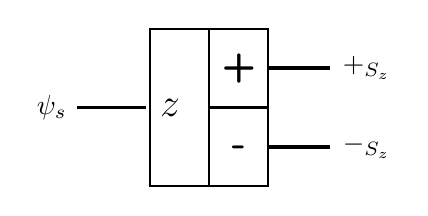
\begin{tikzpicture}[shorten >=1pt,auto, thick,
     square node/.style={rectangle, minimum height=2cm, minimum width=1.50cm, text width = 1.25cm, draw, font=\sffamily\Large\bfseries},
     port/.style={rectangle, draw,  minimum height=1cm, minimum width=0.75cm, font=\sffamily\Large\bfseries},
     wf/.style={rectangle, minimum height=1cm}]
    \apparatus{1}{2}{0}{$z$};

    \node(w0) at (0,0) {$\ket{\psi_s}$};
    \node[wf] (w1) at (4, 0.5) {$\ket{+_{S_z}}$};
    \node[wf] (w2) at (4, -0.5) {$\ket{-_{S_z}}$};

    % \node(label1) at (0, -1.75) {$\bm{t_0}$};
    % \node(label2) at (6.25, -1.75) {$\bm{t_1}$};

    \draw[line width=0.5mm] (w0) -- (1);
    \draw[line width=0.5mm] (1+) -- (w1);
    \draw[line width=0.5mm] (1-) -- (w2);
\end{tikzpicture}

\caption[Insert an abbreviated caption here to show in the List of Figures]
{Stern-Gerlach Experiment 1 as described by the Copenhagen description of measurement. Each measurement outcome }
\label{Figure:Measurement:Copenhagen Experiment 1}
\end{figure}

The Born Rule gives the probabilities of measuring spin-up and spin-down as a function of initial spin state:
\begin{align}
  \mathcal{P}(\pm) = |\braket{\pm | \psi_s}|^2
\end{align}

\subsection{Experiment 2} \label{standard consecutive measurements}

\begin{figure}
\centering\CaptionFontSize
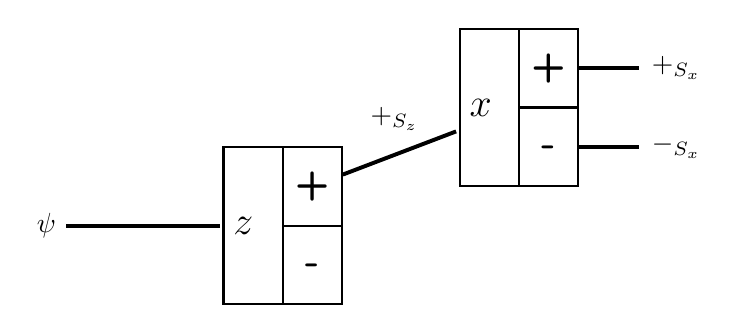
\begin{tikzpicture}[shorten >=1pt,auto, thick,
     square node/.style={rectangle, minimum height=2cm, minimum width=1.50cm, text width = 1.25cm, draw, font=\sffamily\Large\bfseries},
     port/.style={rectangle, draw,  minimum height=1cm, minimum width=0.75cm, font=\sffamily\Large\bfseries},
     wf/.style={rectangle, minimum height=1cm}]
    \apparatus{1}{3}{0}{$z$};
    \apparatus{2}{6}{1.5}{$x$};

    \node[wf] (w0) at (0,0) {$\ket{\psi}$};
    \node[wf] (w1) at (8, 2.0) {$\ket{+_{S_x}}$};
    \node[wf] (w2) at (8, 1.0) {$\ket{-_{S_x}}$};

    \draw[line width=0.5mm] (w0) -- (1);

    \draw[line width=0.5mm] (1+) -- (2) node [near end] {$\ket{+_{S_z}}$};

    \draw[line width=0.5mm] (2+) -- (w1);
    \draw[line width=0.5mm] (2-) -- (w2);
\end{tikzpicture}
\caption[Insert an abbreviated caption here to show in the List of Figures]
{The Stern-Gerlach experiment as described by the standard measurement scheme. Notice that each measurement outcome is renormalized, so that information about the state prior to measurement is lost.}
\label{Figure:Measurement:Copenhagen Experiment 2}
\end{figure}

Now we consecutively measure spin as shown in \autoref{Figure:Measurement:Copenhagen Experiment 2}. The first apparatus serves as a state preparation device, since we are only interested in particles exiting the spin-up output. Using the projection postulate, the state after the first measurement is
\begin{align}
    \ket{\psi^\prime} &= \frac{{P^{S_z}_+}\ket{\psi}}{\sqrt{\bra{\psi}P^{S_z}_+\ket{\psi}}} = \ket{+_{S_z}}
\end{align}
Similarly, the possible output states from the second apparatus are
\begin{align}
  \ket{\psi^{\prime\prime}} &= \frac{P^{S_x}_+\ket{+_{S_z}}}{\sqrt{\bra{+_z}P^{S_x}_+\ket{+_{S_z}}}} = \ket{+_{S_x}}
\end{align}
or
\begin{align}
  \ket{\psi^{\prime\prime}} &= \frac{P^{S_x}_-\ket{+_{S_z}}}{\sqrt{\bra{+_z}P^{S_x}_-\ket{+_{S_z}}}} = \ket{-_{S_x}}
\end{align}

Because we ignore spin-down particles from the first measurement, we are certain that particles entering the second analyzer are in the spin-up state. The probabilities assigned to each state leaving the $S_x$ Stern-Gerlach device are
\begin{align} \label{eq:standard conditional probabilites}
    \mathcal{P}(+_x) &= |\braket{+_{S_x}|+_{S_z}}|^2 = \frac{1}{2} \\ \nonumber
    \mathcal{P}(-_x) &= |\braket{-_{S_x}|+_{S_z}}|^2 = \frac{1}{2}
\end{align}

\section{Dynamics}
In a mechanical theory, the equations of motion (or \textit{dynamics}) describe how a state evolves with time. In classical Newtonian mechanics, this is given by Newton's law of motion
\begin{align}
  \vec{F} = m\vec{a}.
\end{align}

These dynamics are \textit{unitary}, meaning that given the final state of a physical process, the corresponding initial state is recovered by applying the dynamics with time reversed. The dynamics can be represented by a one-to-one map from initial to final states.

The projection postulate describes one type of dynamics, which apply only during measurement. When applied, all information about the initial state is lost as the state instantaneously becomes an eigenstate of the measured variable. The map from initial to final states is not one-to-one; ``collapse dynamics'' are non-unitary.

Quantum theory postulates an another type of dynamics that is analogous to Newton's law of motion. These dynamics are unitary, and apply at all times (not just during measurement).

\invisiblesubsubsection{Postulate 6 (Unitary Dynamics)}
\begin{Thm:Postulate}{6}
  TODO write Schrödinger equation
\end{Thm:Postulate}

\chapter{Measurement}

TODO: chapter preview

State collapse requires extra assumption, ambiguous defs lead to interepretation issues, arrow of time

\section{Issues with State Collapse}

The projection postulate introduces foundational assumptions to describe the measurement process. The principle of Occam's razor says that, in general, a theory is strengthened by making as few assumptions as possible. In classical mechanics, there are no foundational assumptions made to describe measurement; this motivates the pursuit to describe quantum measurement without using the projection postulate.

Furthermore, the projection postulate relies on ambiguous definitions. State collapse occurs upon ``interaction with a classical measuring apparatus'', yet there is no specification of what makes a system classical. Classical systems are not described by the theory, yet they play a fundamental role in the measurement process.

TODO: describe interpretational issues

% This ambiguity makes quantum mechanics exploitable for justification of anthropocentric statements. Examples are widespread in both popular and scientific literature. In the 1975 bestseller \textit{The Tao of Physics},
% \begin{quote}
%  ``The human observer constitutes the final link in the chain of observational processes, and the properties of any atomic object can only be understood in terms of the object's interaction with the observer.'' \cite{Capra}
% \end{quote}
% Similarly, the von Neumann-Wigner interpretation of quantum mechanics asserts that
% \begin{quote}
%  ``[t]here exist external observers which cannot be treated within quantum mechanics, namely human (and perhaps animal) minds, which perform measurements on the brain causing wave function collapse.'' (Schreiber's description of the von Neumann–Wigner interpretation \cite{Schreiber}).
% \end{quote}
%
% This attitude towards quantum measurement prompted Einstein to ask a colleague if they believed that the moon existed only when they looked at it \cite{Pais}. In this thesis, we assert that the moon does exist, even when not directly observed by a human. Instead, we allow a multitude of non-living systems to continuously ``measure'' the moon. This is done using the \textit{von Neumann measurement scheme}, which describes measurement as a physical process involving two quatum systems, neither of which need be human or a ``classical measuring apparatus''.

Because the measurement process cannot be reversed, state collapse injects time asymmetry into the foundations of quantum mechanics. TODO: discuss arrow of time.

The issues with interpretation of state collapse and non-unitary dynamics in general are indicators that collapse dynamics are formulated with ignorance of some underlying process. To begin describing this process, we discard the projection postulate and describe measurement using dynamics permitted by the Schrödinger equation.

Describing measurement as a unitary process is desirable for multiple reasons:
\begin{itemize}
  \item less fundamental assumptions
  \item Humans and measurement apparatuses do not play a special role indescribale by the theory
  \item interpretational issues are circumvented
  \item With dynamics symmetric in time, the emergence of the ``arrow of time'' can be studied
  \item TODO: describe cosmology benefit.
\end{itemize}

Fortunately, such a description is possible using the von Neumann measurement scheme.

\section{von Neumann Measurement Scheme}
In the discussion of Stern-Gerlach experiments, the position of the electron played an implicit role in measurement. In exemplifying use of the \hyperref[projection postulate]{projection posulate} TODO, we define a measurement result as the localization of the electron in the spin-up or spin-down regions. The primary measurement is that of position, which is used to imply the spin state, yet position as a system is never formalized.

Our goal is to formalize the correlation of position and spin eigenstates observed in Stern-Gerlach experiments. We start by representing the electron with a composite spin-position system,
\begin{align}
  \mathcal{H} = \mathcal{H}_s \otimes \mathcal{H}_\mathcal{X}
\end{align}

To exemplify use of the measurement scheme, we revisit Experiment 1. Reaclling TODO REF, the result of the experiment is determined by the final location of the electron; spin-up and spin-down particles are deflected in opposing directions to different ``outputs'' of the analyzer. We name position states of interest; $\ket{\varnothing_\mathcal{X}}$ represents the localization at the beginning of the analyzer (which we call the ``ready'' position), while $\ket{+_{\mathcal{X}}}$ and $\ket{-_{\mathcal{X}}}$ represent localization at the spin-up and spin-down output regions, respectively. Numerous papers detail these position states in terms of Gaussian wave packets \cite{Venugopalan}, but for simplicity we leave them abstracted. It is the purpose of the Stern-Gerlach experiment to seperate spin-up and spin-down particles into spatially distinct regions, so we assert that the named position states are mutually orthonormal:
\begin{align}
  \braket{i_\mathcal{X}| j_\mathcal{X}} &= \delta_{i,j}
\end{align}

We introduce an operator that correlates the position states with spin eigenstates in explicit form:
\begin{align} \label{eq: Experiment 1 unitary operator}
  U(t_1, t_0) &= P^{S_z}_+ \otimes \left(\: \ket{+_{\mathcal{X}}}\bra{\varnothing_\mathcal{X}} \: \bm{+} \: \ket{\varnothing_\mathcal{X}}\bra{+_\mathcal{X}} \: \bm{+} \: I_\mathcal{X} \: \bm{-} \: P^\mathcal{X}_+  \: \bm{-} \: P^\mathcal{X}_\varnothing \: \right) \\ \nonumber
  &\phantom{{}={}} + P^{S_z}_- \otimes \left( \: \ket{-_{\mathcal{X}}}\bra{\varnothing_\mathcal{X}} \: \bm{+} \: \ket{\varnothing_\mathcal{X}}\bra{-_\mathcal{X}} \: \bm{+} \: I_\mathcal{X} \: \bm{-} \: P^\mathcal{X}_-  \: \bm{-} \: P^\mathcal{X}_\varnothing \: \right)
\end{align}

The $P^{S_z}_\pm$ component selects the up or down spin state, while the corresponding $H_\mathcal{X}$ component correlates the $\pm$ position states. The $\ket{\pm_\mathcal{X}}\bra{\varnothing_\mathcal{X}}$ term maps the ``ready'' position state with the up or down position state, while the $I_\mathcal{X} - P^\mathcal{X}_\pm - P^\mathcal{X}_\varnothing$ terms leave position states distinct from $\ket{\pm_\mathcal{X}}$ and $\ket{\varnothing_\mathcal{X}}$ unaffected.

Starting with a general spin state, the final state is
\begin{align} \label{eq: Experiment 1 final state}
  U(t_1, t_0)\ket{\psi} & =  U(t_1, t_0) \left(\ket{\psi_s} \otimes \ket{\varnothing_\mathcal{X}} \right) \\
  &= \nonumber P^{S_z}_+ \ket{\psi_s} \otimes \ket{+_{\mathcal{X}}} \: \bm{+} \: P^{S_z}_- \ket{\psi_s} \otimes \ket{-_{\mathcal{X}}}
\end{align}

At the instant measurement begins $t_0$, the position state is $\ket{\varnothing_\mathcal{X}}$ as the electron enters the magnetic field. At the instant measurement ends $t_1$, the position state is either $\ket{+_{\mathcal{X}}}$ or $\ket{-_{\mathcal{X}}}$, realized with spin-up and spin-down spin states respectively. Notice that the final sum does not contain any terms representing incorrect correlations between spin and position states (such as $ P^{S_z}_+ \ket{\psi_s} \otimes \ket{-_{\mathcal{X}}}$). The presence of these terms would suggest that spin-up particles could be found in the spin-down region, or vice versa; if spin state cannot be deduced from the position state, then a good measurement has not been made. The absence of these terms means that we can deduce the spin state from the position state. Furthermore, the final state cannot be written as the tensor product of a state in $\mathcal{H}_s$ and a state in $\mathcal{H}_\mathcal{X}$ (as the inital state was). This is the definition of \textit{entanglement}; the von Neumann measurement scheme describes the measurement process as entanglement of two independent systems.

The von Neumann scheme is usually written as a linear map:
\begin{align} \label{eq: general final state}
    \nonumber U(t_1, t_0): \\
    & \ket{\psi} = \left(\sum_{n} P^{S_z}_n\ket{\psi_s}\right) \otimes \ket{\varnothing_\mathcal{X}} \mapsto \sum_{n}\left(P^{S_z}_n\ket{\psi_s} \otimes \ket{n_\mathcal{X}}\right)
\end{align}
where $n = +, -$.

Notice that the initial state is a single tensor product, while the final state is a sum of tensor products. The coherence initially present only in the spin state is extended to the composite spin-momentum system. This process is represented schematically in \autoref{Figure:vnm experiment 1}; the initial state branches into two distinct outcomes, each represented by a term in the final state.

\begin{figure}
\centering\CaptionFontSize
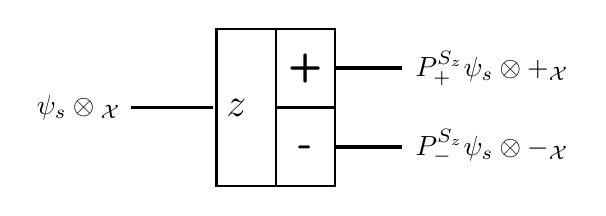
\begin{tikzpicture}[shorten >=1pt,auto, thick,
     square node/.style={rectangle, minimum height=2cm, minimum width=1.50cm, text width = 1.25cm, draw, font=\sffamily\Large\bfseries},
     port/.style={rectangle, draw,  minimum height=1cm, minimum width=0.75cm, font=\sffamily\Large\bfseries},
     wf/.style={rectangle, minimum height=1cm}]
    \apparatus{1}{2}{0}{$z$};

    \node(w0) at (-0.5,0) {$\ket{\psi_s} \otimes \ket{\varnothing_\mathcal{X}}$};
    \node[wf] (w1) at (4.75, 0.5) {$P^{S_z}_+\ket{\psi_s} \otimes \ket{+_{\mathcal{X}}}$};
    \node[wf] (w2) at (4.75, -0.5) {$P^{S_z}_-\ket{\psi_s} \otimes \ket{-_{\mathcal{X}}}$};

    % \node(label1) at (0, -1.75) {$\bm{t_0}$};
    % \node(label2) at (6.25, -1.75) {$\bm{t_1}$};

    \draw[line width=0.5mm] (w0) -- (1);
    \draw[line width=0.5mm] (1+) -- (w1);
    \draw[line width=0.5mm] (1-) -- (w2);
\end{tikzpicture}

\caption[Insert an abbreviated caption here to show in the List of Figures]
{The Stern-Gerlach experiment as described by the von Neumann measurement scheme. Each measurement outcome corresponds to a term in the time-evolved state (\autoref{eq: Experiment 1 final state}). Notice that the measurement interaction results in a branching structure, which is recapitulated spatially by the Stern-Gerlach experiment.}
\label{Figure:vnm experiment 1}
\end{figure}

\section{Preferred Basis Problem}

By describing measurement as a unitary process, we have eliminated many aspects of the quantum measurement problem. TODO cite specific examples. However, there are two overarching problems with interpretation of the entangled state resulting from the von Neumann measurement scheme. These are called the \textit{preferred basis problem} and the \textit{problem of outcomes} in literature \cite{Schlosshauer}\cite{Wang}. A potential solution includes interaction with the environment in the measurement model, and uses tools developed in this thesis so far. The problem of outcomes remains an open research question, and potential solutions lay outside the scope of this thesis.

The preferred basis problem arises from the ability to write the final state in \autoref{eq: general final state} in the same form, but using a different basis:
\begin{align}  \label{eq: preferred basis state general}
  \ket{\psi'} = \sum_{n}\left(P^{S_z}_n\ket{\psi_s} \otimes \ket{n_\mathcal{X}}\right) = \sum_{n}\left({P^{S_z}_{n}}' \ket{\psi_s} \otimes \ket{{n_\mathcal{X}}'}\right) =...
\end{align}

Such a case is exemplified using Experiment 1. Consider setting the initial spin state to spin-up in the $x$ direction:
\begin{align}
  \ket{\psi_s} = \ket{+_{S_x}} = \frac{\ket{+_{S_z}} + \ket{-_{S_z}}}{\sqrt{2}}
\end{align}

The final state by \autoref{eq: Experiment 1 unitary operator} is
\begin{align} \label{eq:preferred basis state z}
  \ket{\psi'} = \frac{\ket{+_{S_z}}\otimes\ket{+_{\mathcal{X}}} + \ket{-_{S_z}}\otimes\ket{-_{\mathcal{X}}}}{\sqrt{2}}
\end{align}

Similar to the $S_x$ eigenstates, we define orthonormal position states
\begin{align}
  \ket{+_{\mathcal{X}_x}} = \frac{\ket{+_{\mathcal{X}}} + \ket{-_{\mathcal{X}}}}{\sqrt{2}} \\ \nonumber
  \ket{-_{\mathcal{X}_x}} = \frac{\ket{+_{\mathcal{X}}} - \ket{-_{\mathcal{X}}}}{\sqrt{2}}
\end{align}

so that the final state can be written
\begin{align} \label{eq:preferred basis state x}
  \ket{\psi'} &= \frac{ \left(\frac{\ket{+_{S_x}} + \ket{-_{S_x}}}{\sqrt{2}} \otimes \frac{\ket{+_{\mathcal{X}_x}} + \ket{-_{\mathcal{X}_x}}}{\sqrt{2}} \right) +  \left(\frac{\ket{+_{S_x}} - \ket{-_{S_x}}}{\sqrt{2}} \otimes \frac{\ket{+_{\mathcal{X}_x}} - \ket{-_{\mathcal{X}_x}}}{\sqrt{2}} \right) }{\sqrt{2}} \\ \nonumber
  \ket{\psi'} &= \frac{\ket{+_{S_x}} \otimes \ket{+_{\mathcal{X}_x}} + \ket{-_{S_x}} \otimes \ket{-_{\mathcal{X}_x}}}{\sqrt{2}}
\end{align}

\autoref{eq:preferred basis state x} matches \autoref{eq:preferred basis state z} in form; it appears that the measurement process of spin along the $z$ axis has entangled orthonormal position states with spin states along the $x$ axis. If we regard such an entanglement as the measurement process, the von Neumann measurement scheme violates the princple of complementarity by simultaneously measuring $S_z$ and $S_x$. We know the experimental setup was configured to measure $S_z$, but nothing in the theory singles out $S_z$ as the \textit{preferred basis}.

Returning to the general problem \autoref{eq: preferred basis state general}, we note that $\{ \ket{n_s} \}$ and $\{ \ket{n_\mathcal{X}} \}$ are orthogonal sets, so $\ket{\psi'}$ is a biorthogonal system. The biorthogonal decomposition theorem states that alternate bases $\{ \ket{n'_s} \}$ and $\{ \ket{n'_\mathcal{X}} \}$ satisfying \autoref{eq: preferred basis state general} exist when $\braket{n_s | \psi_s}$ are not all distinct \cite{Elby}. Limiting this condition to normalized states of spin-$\frac{1}{2}$ systems, states with coefficients $\braket{n_s | \psi_s} = \frac{1}{\sqrt{2}}$ for both $n = +$ and $n = -$ are subject to the preferred basis problem as shown. Since every state in $\mathcal{H}$ can be expressed in this form by expansion in the pertinent basis, the system is always subject to the preferred basis problem.

\section{Einselection}

While systems in the form \autoref{eq: general final state} do not generally have unique decompositions, systems with three or more components do by the triorthogonal decomposition theorem, so long as all three components are expanded in two orthogonal (and one non-colinear) bases \cite{Elby}. We open the spin-position system to interaction with some third system $\mathcal{H}_\epsilon$. Asserting that during measurement, $\ket{\psi_\epsilon}$ is entangled with the $\ket{\psi_s}$ just as $\ket{\psi_\mathcal{X}}$ is entangled with $\ket{\psi_s}$,
\begin{align} \label{eq:selected basis}
  \ket{\psi'} = \sum_{n}\left(P^{S_z}_n\ket{\psi_s} \otimes \ket{n_\mathcal{X}} \otimes \ket{n_\epsilon} \right) \neq \sum_{n}\left({P^{S_z}_n}'\ket{\psi_s} \otimes \ket{{n_\mathcal{X}}'} \otimes \ket{{n_\epsilon}'} \right).
\end{align}
Since there is no other basis into which $\ket{\psi'}$ can expand to this form, the preferred basis has been selected by including a third system that also undergoes von Neumann measurement. But what is this system?

For guidance, we look back to the original phrasing of the von Neumann measurement scheme, where measurement is described as the entanglement of a microscopic system with a macroscopic measuring apparatus \cite{Neumann}. Many descriptions of Stern-Gerlach measurement interpret the electron position system as the apparatus itself \cite{Venugopalan}. This is a reasonable abstraction, as the position of the electron is used to ``read off'' the result of the measurement. However, this approach is misleading, because it conflates two distinct physical systems; the apparatus, and the position system belonging to the electron. By labeling the position system as the ``apparatus'', the degree of freedom corresponding to the actual apparatus is effectively ignored.

Newton's third law asserts that an interaction consists of equal and opposite actions between two systems. For the Stern-Gerlach experiment, the interaction between the analyzer magnet and the electron affects both the electron and the magnet, yet we have only described the effect on the electron. An approach to the preferred basis problem interprets the third system $H_\epsilon$ as the apparatus, so that \autoref{eq:selected basis} also describes the effect on the magnet from the interaction. Selecting a basis by acknowledging the hidden degree of freedom for the apparatus has been proposed under the name \textit{interaction induced superselection} (or \textit{inselection})\cite{Wang}.

A much more established approach interprets the third system as the \textit{environment}, which consists of every imaginable system other than the electron. This approach is called \textit{environment induced superselection} or \textit{einselection}. Imagine every system that collides with the electron (gas molecules, photons, ...); the collision's occurrence depends on the electron's trajectory (which is dependent on its spin). Given omnipotent knowledge of every system's interaction with the electron, one could deduce its spin state. When the electron is realized with spin-up or spin-down, there are causal effects in the environment that encode the electron's history; we say that the environment continuously records \textit{which-state information} about the system \cite{Schlosshauer}. We can think of the environment as constantly interacting with our system to establish the ``facts of the universe'' about the electron.

Because the environment necessarily includes the apparatus, the
Rather than framing inselection as a different approach from einselection, we suggest that it describes a mechanism of basis selection that is comptabile with (but more precise than) einselection. Because the environment includes all other systems interacting with the electron, the interaction with the basis e inclusion of the apparatus (which \textit{must} exist by Newton's third law) selects a basis


Ein is more established, includes added benefit of record keeping. We discussed inselection to introduce how extending entanglement to  environment works

A suggested approach argues that \autoref{eq: general final state} fails to account for the entanglement of the measuring apparatus with the electron. \autoref{eq: general final state} accounts for the effect of the  Newton's third law tells us that the force exerted on the electron by the apparatus magnet is paired with a force exerted on the magnet by the electron. While we can describe the effect on the electron using $\ket{\psi_s} \otimes \ket{\psi_\mathcal{X}}$, we

How could this go unnoticed? Perhaps because previous explanatoin suck. Not well established, but ...
If something that must exist solves the preferred basis problem, it is more precise to say that it does vs something that. Inselection could be  a more precise mechanism that is normally obscured in einselection.

 Selection of the preferred basis problem by formalizing the system-environment interaction is called \textit{environment induced superselection} or \textit{einselection} \cite{Zurek}.

We now formalize the spin-position-environment interaction, similar to how the spin-position correlation implied in the projection postulate was formalized. We name $\ket{\varnothing_\epsilon}$ representing the environment's recording of the apparatus in the ready state only, and $\ket{\pm_\epsilon}$ representing the environment's recording of the apparatus in spin-up or spin-down. Representing classically distinct outcomes, we assert orthonormality
\begin{align}
  \braket{i_\epsilon | j_\epsilon} = \delta_{i,j}
\end{align}
for $i,j = \varnothing, +, -$.
Idealizing the environment as a perfect record keeper, the dynamics must map
\begin{align} \label{eq: unitary operator inselection}
    \nonumber U(t_1, t_0): \\
    & \ket{\psi} = \left(\sum_{n} P^{S_z}_n\ket{\psi_s}\right) \otimes \ket{\varnothing_\mathcal{X}} \otimes \ket{\varnothing_\epsilon} \mapsto \sum_{n}\left(P^{S_z}_n\ket{\psi_s} \otimes \ket{n_\mathcal{X}} \otimes \ket{n_\epsilon} \right)
\end{align}
where $n= +,-$.

\subsection{Experiment 1}
Our system is now composed of spin, position, and environment systems $H = H_s \otimes H_\mathcal{X} \otimes H_\epsilon$. The unitary operator satisfying \autoref{eq: unitary operator inselection} is
\begin{align}
  U(t_1, t_0) &= P^{S_z}_+ \otimes \left(\: \ket{+_{\mathcal{X}}}\bra{\varnothing_\mathcal{X}} \: \bm{+} \: \ket{\varnothing_\mathcal{X}}\bra{+_\mathcal{X}} \: \bm{+} \: \ket{-_{\mathcal{X}}}\bra{-_\mathcal{X}} \: \bm{+} \: I_\mathcal{X} \: \bm{-} \: P^\mathcal{X}_+  \: \bm{-} \: P^\mathcal{X}_\varnothing \: \right) \\ \nonumber
  &\phantom{{}=P^{S_z}_+} \otimes \left(\: \ket{+_\epsilon}\bra{\varnothing_\epsilon} \: \bm{+} \: \ket{\varnothing_\epsilon}\bra{+_\epsilon} \: \bm{+} \: \ket{-_\epsilon}\bra{-_\epsilon} \: \bm{+} \: I_\epsilon \: \bm{-} \: P^\epsilon_+  \: \bm{-} \: P^\epsilon_\varnothing \: \right)\\ \nonumber
  &+ P^{S_z}_- \otimes \left( \: \ket{-_{\mathcal{X}}}\bra{\varnothing_\mathcal{X}} \: \bm{+} \: \ket{\varnothing_\mathcal{X}}\bra{-_\mathcal{X}} \: \bm{+} \: \ket{+_{\mathcal{X}}}\bra{+_\mathcal{X}} \: \bm{+} \: I_\mathcal{X} \: \bm{-} \: P^\mathcal{X}_-  \: \bm{-} \: P^\mathcal{X}_\varnothing \: \right) \\ \nonumber
 &\phantom{{}=P^{S_z}_-} \otimes \left(\: \ket{-_\epsilon}\bra{\varnothing_\epsilon} \: \bm{+} \: \ket{\varnothing_\epsilon}\bra{-_\epsilon} \: \bm{+} \: \ket{+_\epsilon}\bra{+_\epsilon} \: \bm{+} \: I_\epsilon \: \bm{-} \: P^\epsilon_-  \: \bm{-} \: P^\epsilon_\varnothing \: \right)
\end{align}

To shorten this expression, we define the ``entanglement operator''
\begin{align}
  E^i_{\pm, \varnothing} &= \ket{\pm_i}\bra{\varnothing_i} \: \bm{+} \: \ket{\varnothing_i}\bra{\pm_i} \: \bm{+} \: \ket{\mp_i}\bra{\mp_i} + I_i - P^i_\pm - P^i_\mp
\end{align}

Note that $E$ is Hermitian $\left(E^\dagger = E\right)$ and unitary $\left( E^\dagger E = I \right)$. The unitary operator is now
\begin{align}  \label{einselection experiment 1}
  U(t_1, t_0) &= P^{S_z}_+ \otimes E^\mathcal{X}_{+, \varnothing} \otimes E^\epsilon_{+,\varnothing} \\ \nonumber
  &+ P^{S_z}_- \otimes E^\mathcal{X}_{-, \varnothing} \otimes E^\epsilon_{-, \varnothing}
\end{align}

For a general initial spin state, this produces final state
\begin{align}
  \ket{\psi'} &= P^{S_z}_+ \ket{\psi_s} \otimes \ket{+_{\mathcal{X}}} \otimes \ket{+_\epsilon} \: \bm{+} \: P^{S_z}_- \ket{\psi_s} \otimes \ket{-_{\mathcal{X}}} \otimes \ket{-_\epsilon}
\end{align}
This experiment is visualized schematically in \autoref{fig: Experiment 1 inselection}.

\begin{figure}
\centering\CaptionFontSize
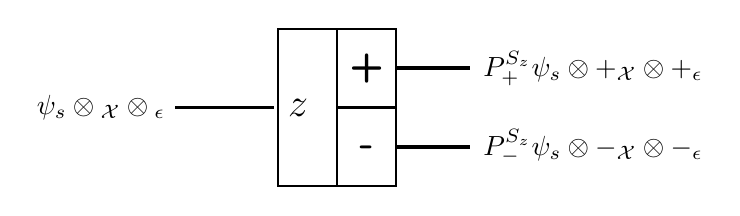
\begin{tikzpicture}[shorten >=1pt,auto, thick,
     square node/.style={rectangle, minimum height=2cm, minimum width=1.50cm, text width = 1.25cm, draw, font=\sffamily\Large\bfseries},
     port/.style={rectangle, draw,  minimum height=1cm, minimum width=0.75cm, font=\sffamily\Large\bfseries},
     wf/.style={rectangle, minimum height=1cm}]
    \apparatus{1}{2}{0}{$z$};

    \node(w0) at (-1,0) {$\ket{\psi_s} \otimes \ket{\varnothing_\mathcal{X}} \otimes \ket{\varnothing_\epsilon}$};
    \node[wf] (w1) at (5.25, 0.5) {$P^{S_z}_+\ket{\psi_s} \otimes \ket{+_{\mathcal{X}}} \otimes \ket{+_\epsilon}$};
    \node[wf] (w2) at (5.25, -0.5) {$P^{S_z}_-\ket{\psi_s} \otimes \ket{-_{\mathcal{X}}} \otimes \ket{-_\epsilon}$};

    % \node(label1) at (0, -1.75) {$\bm{t_0}$};
    % \node(label2) at (6.25, -1.75) {$\bm{t_1}$};

    \draw[line width=0.5mm] (w0) -- (1);
    \draw[line width=0.5mm] (1+) -- (w1);
    \draw[line width=0.5mm] (1-) -- (w2);
\end{tikzpicture}
\caption[Insert an abbreviated caption here to show in the List of Figures]
{The most complete description of Experiment 1 presented, including position and environment degres of freedom. The seemingly redundant correlation of both position and environment states to spin states validifies the abstraction of the apparatus as the position system. However, formalizing the interaction with the apparatus, and more generally the environment, resolves the preferred basis problem and provides a description of record keeping.}
\label{fig: Experiment 1 inselection}
\end{figure}

\section{Consecutive Measurements}

In \autoref{standard consecutive measurements}, we applied the projection postulate succesively to account for consecutive measurements. When measurement was conditional on a prior result, we applied the postulate only to states routed to the second analyzer. The von Neumann measurement scheme can also be applied succesively, and is used on a term-by-term basis to account for conditional measurement.

\subsection{Experiment 2}
Now the environment must record the state of two apparatuses. To simplify this, we seperate the components of the environment responsible for recording each apparatus
\begin{align}
  H_\epsilon = H_{\epsilon_1} \otimes H_{\epsilon_2}
\end{align}

so that the complete Hilbert space is
\begin{align}
  \mathcal{H} = \mathcal{H}_s \otimes \mathcal{H}_\mathcal{X} \otimes \mathcal{H}_{\epsilon_1} \otimes \mathcal{H}_{\epsilon_2}
\end{align}
We also name new position states for the second apparatus, so that position states of interest are now $\{ \ket{\varnothing_{\mathcal{X}}^1}, \ket{+_{\mathcal{X}}^1}, \ket{-_{\mathcal{X}}^1}, \ket{\varnothing_{\mathcal{X}}^2}, \ket{+_{\mathcal{X}}^2}, \ket{-_{\mathcal{X}}^2} \}$. These states are visualized in TODO FIG.

The dynamics are unchanged from \autoref{einselection experiment 1} for the first measurement, with the identity acting on the second environment system to leave it unaffected:
\begin{align}
  U(t_1, t_0) &= P^{S_z}_+ \otimes E^{\mathcal{X}}_{+^1, \varnothing^1}  \nonumber \otimes E^{\epsilon_1}_{+, \varnothing} \otimes I_{\epsilon_2}\\ \nonumber
  &+ P^{S_z}_- \otimes E^{\mathcal{X}}_{-^1, \varnothing^1} \otimes E^{\epsilon_1}_{-,\varnothing} \otimes I_{\epsilon_2}
\end{align}

For the second measurement, we begin by selecting $z$ spin-down states and leave them unaffected
\begin{align}
  U(t_2, t_1) &=  P^{S_z}_- \otimes I_\mathcal{X} \otimes I_{\epsilon_1} \otimes I_{\epsilon_2}
\end{align}
Then, we select $z$ spin-up states and perform the measurement scheme again, since these are routed to the second analyzer.
\begin{align}
  U(t_2, t_1) &= P^{S_x}_+ P^{S_z}_+ \otimes E^\mathcal{X}_{+^2, +^1} \otimes I_{\epsilon_1} \otimes E^{\epsilon_2}_{+, \varnothing} \\ \nonumber
  &+ P^{S_x}_- P^{S_z}_+ \otimes E^\mathcal{X}_{+^2, -^1} \otimes I_{\epsilon_1} \otimes E^{\epsilon_2}_{-, \varnothing} \\ \nonumber
  &+ P^{S_z}_- \otimes I_\mathcal{X} \otimes I_{\epsilon_1} \otimes I_{\epsilon_2}
\end{align}
The $\epsilon_2$ entanglement operator functions just as the $\epsilon_1$ operator did for the first measurement. The position entanglement operator is more subtle. Immediately after the first measurement, we expect the up and down position state to be mapped to the ready state of the second analyzer. Immediately after that, the ready state is mapped to up and down position states as the second measurement takes place. Considering both of these mappings as the second measurement, we directly map up/down position states from the first analyzer to up/down position states of the second.

Because the environment is used as the third degree of freedom, we do not have to worry about reversing the spin-apparatus entanglement after measurement. The role of the environment is to keep a persistent record, so we let it be.

% \begin{align}
%   U(t_2, t_1) &= U(t_2, t_1)_{a_1} U(t_2, t_1)_{a_2} \\ \nonumber
%   &= P^x_+ P^{S_z}_+ \otimes \left(\ket{+_{a_1}}\bra{\varnothing_{a_1}} \: \bm{+} \: \ket{\varnothing_{a_1}}\bra{+_{a_1}} \: \bm{+} \: \ket{-_{a_1}}\bra{-_{a_1}} \right) \\ \nonumber
%   & \phantom{{} = P^x_+ P^{S_z}_+} \otimes  \left(\ket{+_{a_2}}\bra{\varnothing_{a_2}} \: \bm{+} \: \ket{\varnothing_{a_2}}\bra{+_{a_2}} \: \bm{+} \: \ket{-_{a_2}}\bra{-_{a_2}} \right) \\ \nonumber
%   &+ P^x_- P^{S_z}_+ \otimes \left(\ket{+_{a_1}}\bra{\varnothing_{a_1}} \: \bm{+} \: \ket{\varnothing_{a_1}}\bra{+_{a_1}} \: \bm{+} \: \ket{-_{a_1}}\bra{-_{a_1}} \right) \\ \nonumber
%   & \phantom{{} = P^x_+ P^{S_z}_+} \otimes  \left(\ket{-_{a_2}}\bra{\varnothing_{a_2}} \: \bm{+} \: \ket{\varnothing_{a_2}}\bra{-_{a_2}} \: \bm{+} \: \ket{+_{a_2}}\bra{+_{a_2}} \right) \\ \nonumber
%   &+ P^{S_z}_- \otimes \left(\ket{-_{a_1}}\bra{\varnothing_{a_1}} \: \bm{+} \: \ket{\varnothing_{a_1}}\bra{-_{a_1}} \: \bm{+} \: \ket{+_{a_1}}\bra{+_{a_1}} \right) \\ \nonumber
%   & \phantom{{}={}P^{S_z}_+} \otimes I_{a_2}
% \end{align}

\begin{figure}
\centering\CaptionFontSize

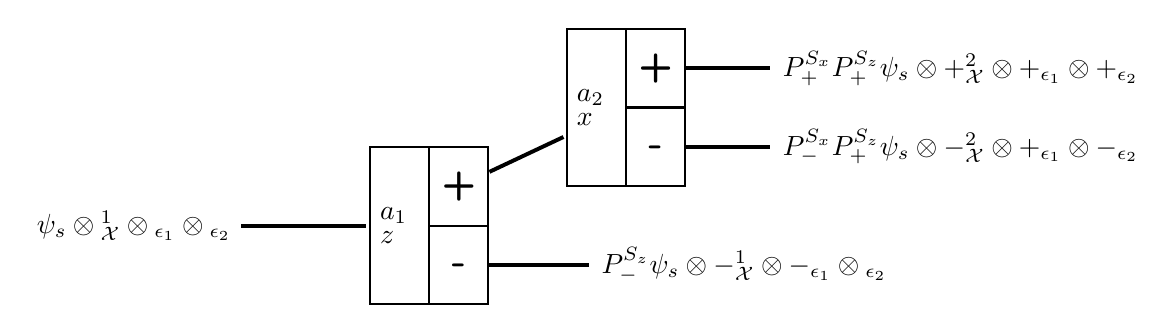
\begin{tikzpicture}[shorten >=1pt,auto, thick,
     square node/.style={rectangle, minimum height=2cm, minimum width=1.50cm, text width = 1.25cm, draw, font=\sffamily\Large\bfseries},
     port/.style={rectangle, draw,  minimum height=1cm, minimum width=0.75cm, font=\sffamily\Large\bfseries},
     wf/.style={rectangle, minimum height=1cm}]
    \apparatus{1}{4}{0}{${}^{a_1}_z$};
    \apparatus{2}{6.5}{1.5}{${}^{a_2}_x$};

    \node(w0) at (0.25,0) {$\ket{\psi_s} \otimes \ket{\varnothing_\mathcal{X}^1} \otimes \ket{\varnothing_{\epsilon_1}} \otimes \ket{\varnothing_{\epsilon_2}} $};
    \node[wf] (w1) at (8, -.5) {$P^{S_z}_-\ket{\psi_s} \otimes \ket{-_{\mathcal{X}}^1}  \otimes \ket{-_{\epsilon_1}} \otimes \ket{\varnothing_{\epsilon_2}}$};
    \node[wf] (w2) at (10.75, 1) {$P^{S_x}_-P^{S_z}_+\ket{\psi}_s \otimes \ket{-_{\mathcal{X}}^2} \otimes \ket{+_{\epsilon_1}} \otimes \ket{-_{\epsilon_2}}$};
    \node[wf] (w3) at (10.75, 2) {$P^{S_x}_+ P^{S_z}_+\ket{\psi_s} \otimes \ket{+_{\mathcal{X}}^2} \otimes \ket{+_{\epsilon_1}} \otimes \ket{+_{\epsilon_2}}$};

    % \node(label0) at (0, -1.75) {$\bm{t_0}$};
    % \node(label1) at (4.75, -1.75) {$\bm{t_1}$};
    % \node(label2) at (7.25, -1.75) {$\bm{t_2}$};
    % \node(label3) at (9.75, -1.75) {$\bm{t_3}$};
    % \node(bw1) at (-1.75, 1.75) {$P^{S_z}_+\ket{\psi}^s \otimes \ket{+_{S_z}}^{D_1}_z \otimes \ket{\varnothing}^{D_2}_\mathcal{X} $};

    \draw[line width=0.5mm] (w0) -- (1);
    \draw[line width=0.5mm] (1+) -- (2);
    \draw[line width=0.5mm] (1-) --  (w1);
    \draw[line width=0.5mm] (2+) -- (w3);
    \draw[line width=0.5mm] (2-) -- (w2);


\end{tikzpicture}

\caption[Insert an abbreviated caption here to show in the List of Figures]
{Schematic of consecutive measurement with spin, position and environment degrees of freedom. Notice the temporary encoding of measurement results in position states, and persistent encoding of measurement results in environment states.}
\label{Figure:Measurement:consecutive final}
\end{figure}
